\chapter{Data Types and Data Quality}
\label{chap:data-quality}
\chapterguide
  {You should be able to load a CSV and inspect its rows, columns, and summaries.}
  {classify variable roles; audit missingness, duplicates, validity, and consistency; and document defensible cleaning decisions.}

\section{Type means more than storage format}
R reports storage classes such as numeric or character, but analysis also depends on measurement meaning.

\begin{dstable}
\begin{tabularx}{\linewidth}{@{}D{2.7cm}D{4.1cm}Y@{}}
\toprule
\rowcolor{DSPaleBlue!92}
\textbf{Analytical type} & \textbf{Example} & \textbf{Appropriate operations} \\
\midrule
Identifier & sample ID & matching, uniqueness checks; not averages \\
Nominal category & species, diagnosis & counts, proportions, group comparisons \\
Ordinal category & low / medium / high & ordered comparisons; spacing is not guaranteed equal \\
Numeric measurement & length, radius & summaries, differences, models \\
Target / outcome & malignant or benign & evaluation against predictions \\
\bottomrule
\end{tabularx}
\end{dstable}

\begin{pitfall}
A number is not automatically quantitative. Student ID 1042 plus Student ID 1043 does not create a meaningful sum. Analytical meaning determines what operations are valid.
\end{pitfall}


\section{Quality is fitness for a specific purpose}
There is no dataset that is simply ``clean'' in the abstract. Quality means that the data are sufficiently accurate, complete, consistent, timely, and appropriately sampled for a particular question. A missing measurement may be harmless for one summary and fatal for another model. A duplicated transaction may be legitimate if the unit of analysis is a transaction, but a serious error if the table is supposed to contain one row per customer.

\begin{utpfig}[Data quality is question-dependent]{The same table can be adequate for one task and inadequate for another because different questions depend on different fields and assumptions.}{fig:quality-purpose}
\begin{tikzpicture}[x=\linewidth,y=1cm,
  sourcecard/.style={draw=UTPBlue!75,fill=UTPPaleBlue,rounded corners=1.8mm,
    line width=0.75pt,text width=0.15\linewidth,
    minimum width=0.19\linewidth,minimum height=1.15cm,
    inner xsep=3mm,inner ysep=2.5mm,align=center,
    font=\scriptsize\color{UTPNavy}},
  taskcard/.style={draw=UTPBlue!65,fill=UTPPaleBlue,rounded corners=1.8mm,
    line width=0.7pt,text width=0.21\linewidth,
    minimum width=0.255\linewidth,minimum height=1.05cm,
    inner xsep=3.5mm,inner ysep=2mm,align=left,
    font=\scriptsize\color{UTPNavy}},
  qualityflow/.style={-{Stealth[length=2mm,width=1.5mm]},
    line width=0.85pt,draw=UTPTeal}]
\node[sourcecard] (data) at (0.12,0)
  {\textcolor{UTPBlue}{\textbf{SHARED INPUT}}\\[3pt]
   The same dataset};
\node[taskcard] (q1) at (0.43,0.80)
  {\textcolor{UTPBlue}{\textbf{QUESTION A}}\\[3pt]
   Requires a complete target.};
\node[taskcard] (q2) at (0.43,-0.80)
  {\textcolor{UTPBlue}{\textbf{QUESTION B}}\\[3pt]
   Requires reliable dates.};
\node[taskcard,draw=UTPTeal!80,fill=UTPPaleTeal] (a1) at (0.78,0.80)
  {\textcolor{UTPTeal}{\textbf{QUALITY CHECK}}\\[3pt]
   Is the target complete and reliable?};
\node[taskcard,draw=UTPTeal!80,fill=UTPPaleTeal] (a2) at (0.78,-0.80)
  {\textcolor{UTPTeal}{\textbf{QUALITY CHECK}}\\[3pt]
   Are the dates complete and valid?};
\coordinate (split) at (0.275,0);
\draw[draw=UTPTeal,line width=0.85pt] (data.east) -- (split);
\draw[qualityflow] (split) |- (q1.west);
\draw[qualityflow] (split) |- (q2.west);
\draw[qualityflow] (q1.east) -- (a1.west);
\draw[qualityflow] (q2.east) -- (a2.west);
\fill[UTPTeal] (split) circle (1.3pt);
\end{tikzpicture}
\end{utpfig}

\section{Four dimensions of a practical data audit}
\begin{utpfig}[Quality audit]{A quality audit asks whether the data are complete enough, internally valid, consistently represented, and uniquely recorded for the intended analysis.}{fig:quality-audit}
\begin{tikzpicture}[x=\linewidth,y=1cm,
  auditroot/.style={draw=UTPTeal!80,fill=UTPPaleTeal,rounded corners=5mm,
    line width=0.75pt,text width=0.17\linewidth,minimum height=0.90cm,
    inner xsep=3mm,inner ysep=2mm,align=center,
    font=\scriptsize\color{UTPNavy}},
  auditcard/.style={draw=UTPBlue!65,fill=UTPPaleBlue,rounded corners=1.8mm,
    line width=0.7pt,text width=0.235\linewidth,
    minimum width=0.29\linewidth,minimum height=1.15cm,
    inner xsep=4mm,inner ysep=2.5mm,align=left,
    font=\footnotesize\color{UTPNavy}},
  auditflow/.style={-{Stealth[length=2mm,width=1.5mm]},
    line width=0.8pt,draw=UTPTeal}]
\node[auditroot] (audit) at (0.50,0)
  {\textbf{QUALITY AUDIT}\\[3pt]
   \color{UTPMuted}fit for purpose};
\node[auditcard] (c) at (0.20,1.00)
  {\textcolor{UTPBlue}{\textbf{01  COMPLETENESS}}\\[4pt]
   Missing values};
\node[auditcard] (v) at (0.80,1.00)
  {\textcolor{UTPBlue}{\textbf{02  VALIDITY}}\\[4pt]
   Plausible ranges};
\node[auditcard] (s) at (0.20,-1.00)
  {\textcolor{UTPBlue}{\textbf{03  CONSISTENCY}}\\[4pt]
   Labels and units};
\node[auditcard] (u) at (0.80,-1.00)
  {\textcolor{UTPBlue}{\textbf{04  UNIQUENESS}}\\[4pt]
   Duplicate records};
\draw[auditflow] (audit.west) to[out=160,in=0] (c.east);
\draw[auditflow] (audit.east) to[out=20,in=180] (v.west);
\draw[auditflow] (audit.west) to[out=200,in=0] (s.east);
\draw[auditflow] (audit.east) to[out=-20,in=180] (u.west);
\end{tikzpicture}
\end{utpfig}


\begin{utpfig}[A row-level quality map]{The deliberately corrupted Iris dataset contains missing and invalid values. A map makes concentration and co-occurrence visible, which a single missing-value count cannot show.}{fig:quality-map}
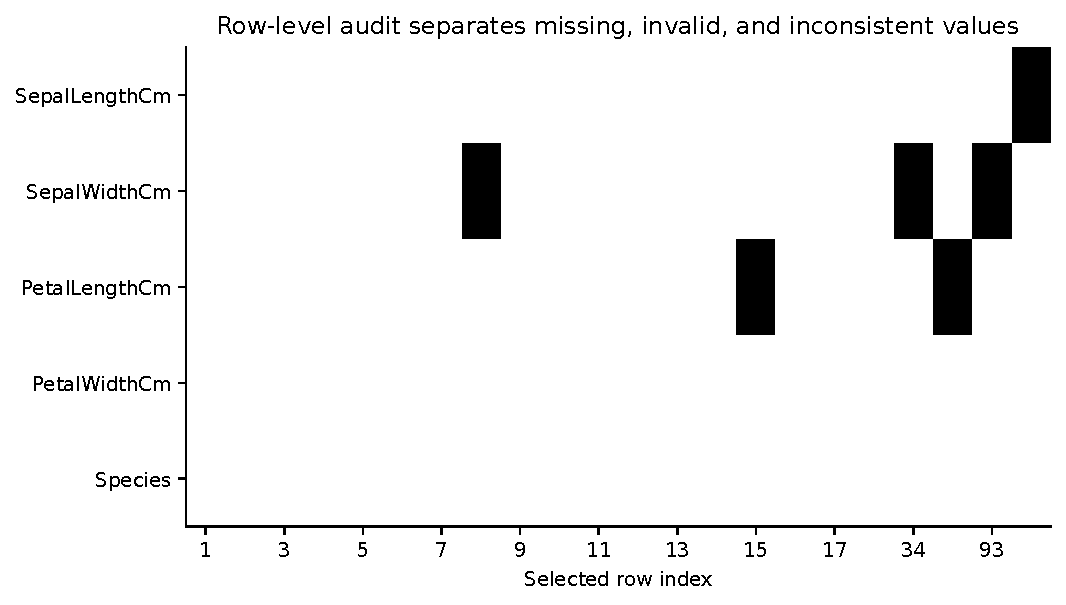
\includegraphics[width=0.93\linewidth]{figures_generated/quality_missingness_map.pdf}
\end{utpfig}


Missingness is not just a count. Ask \emph{which variable is missing, for which records, and whether the absence itself could be informative}. A cleaning rule that is harmless for one question can bias another.

\section{Validity rules come from the domain}
A positive physical length cannot be negative. A probability must lie between 0 and 1. A date of discharge should not precede admission. These are semantic constraints, not software constraints.

\begin{lstlisting}[style=dsr]
invalid <- iris$SepalLengthCm <= 0 |
           iris$SepalWidthCm <= 0
sum(invalid, na.rm = TRUE)
\end{lstlisting}


\section{Missing-data mechanisms change what is defensible}
The cause of missingness matters. Three common conceptual cases are useful:
\begin{itemize}
  \item \textbf{Missing completely at random (MCAR):} absence is unrelated to measured or unmeasured values. Complete-case analysis may remain unbiased, although less precise.
  \item \textbf{Missing at random (MAR):} absence can be explained by observed variables. Conditional imputation or modelling may be defensible if those predictors are included.
  \item \textbf{Missing not at random (MNAR):} absence depends on the missing value itself or another unobserved factor. Sensitivity analysis and domain knowledge become important because the missingness process cannot be repaired mechanically from observed columns alone.
\end{itemize}
These labels are assumptions about the data-generating process, not properties that software can determine with certainty from the table.


\section{Missing data: deletion, imputation, or model explicitly}
There is no universally correct treatment.
\begin{itemize}
  \item \textbf{Delete} when missingness is small and plausibly unrelated to the outcome, and report how many rows were removed.
  \item \textbf{Impute} when preserving rows is important and a defensible replacement rule exists.
  \item \textbf{Model missingness} or add an indicator when the absence itself may carry information.
\end{itemize}

Simple median imputation is robust to extreme values but reduces apparent variability. It is suitable as a teaching method, not a reason to ignore why values are missing.


\begin{utpfig}[Cleaning changes the evidence]{Applying a validity rule can visibly change a distribution. The analyst should compare before and after, count affected rows, and document why the rule is justified.}{fig:quality-cleaning-change}
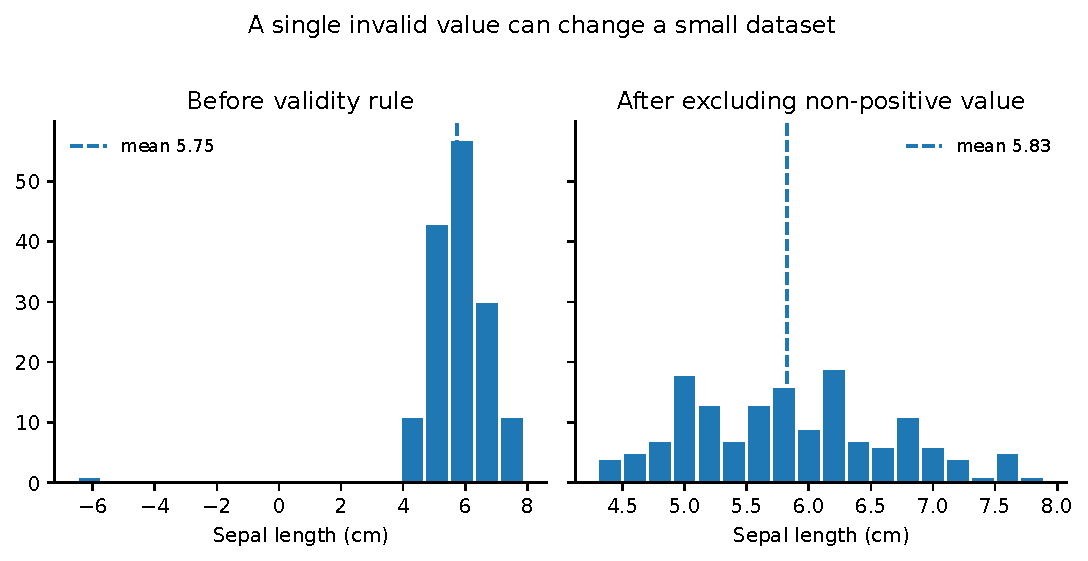
\includegraphics[width=0.82\linewidth]{figures_generated/quality_cleaning_distribution.pdf}
\end{utpfig}

\section{Keys, duplicates, and unit-of-observation errors}
A duplicate is defined relative to an expected key. Exact duplicated rows are easy to find, but more important problems include duplicated identifiers with conflicting values and repeated observations that are legitimate but accidentally treated as independent entities. Before removing anything, determine the intended key and whether repeated keys are expected.

\begin{lstlisting}[style=dsr]
# Are IDs unique when they should be?
anyDuplicated(iris$Id)

# Which IDs repeat?
iris$Id[duplicated(iris$Id)]
\end{lstlisting}

\section{Duplicates and inconsistent categories}
Exact duplicates can inflate counts and train/test performance. Inconsistent labels such as \rcode{"Iris-setosa"}, \rcode{"iris setosa"}, and \rcode{"SETOSA"} represent one concept but appear as three categories until standardised.

\begin{workedexample}
A defensible cleaning log records the rule and the evidence:
\begin{dstable}
\begin{tabularx}{\linewidth}{@{}D{3.2cm}D{4.5cm}Y@{}}
\toprule
\rowcolor{DSPaleBlue!92}
\textbf{Issue} & \textbf{Rule} & \textbf{Evidence retained} \\
\midrule
Duplicate row & keep first exact record & duplicate count before/after \\
Negative length & mark impossible value missing & row identifier and rule \\
Missing measurement & median within species & imputation method and affected count \\
Label variant & normalise case/spacing & original and standard labels \\
\bottomrule
\end{tabularx}
\end{dstable}
\end{workedexample}


\section{Measurement error and label quality}
Not every bad value is impossible. Measurements can be noisy even when they lie in a plausible range, and labels can be incorrect even when they use a valid category name. This distinction matters because a range check finds impossible values but not subtle measurement error.

For supervised learning, target quality is especially important. If diagnosis labels contain errors, the model is trained to reproduce those errors. Apparent model ``mistakes'' may sometimes reveal ambiguous or mislabeled examples rather than algorithm failure.


\section{Leakage: a quality problem for modelling}
\term{Data leakage} occurs when information unavailable at prediction time enters model training. Examples include using a final diagnosis to construct an input feature or scaling the entire dataset before the train/test split. Leakage produces optimistic evaluation, even when the code runs correctly.

\begin{keyidea}
Cleaning is an analytical decision. A good report states what changed, why it changed, how many records were affected, and what uncertainty the change creates.
\end{keyidea}


\begin{utpfig}[Leakage is information arriving from the future]{A modelling feature is legitimate only if it would be available at the moment a real prediction must be made. Post-outcome information can make validation look excellent while making deployment impossible.}{fig:leakage-timeline}
\begin{tikzpicture}[x=1cm,y=1cm]
\draw[-{Stealth[length=2.5mm]},thick,draw=UTPMuted] (-5,0)--(5,0);
\node[tagb] at (-4.1,0.6) {information available};
\node[tagb] at (0,0.65) {prediction time};
\node[tagb] at (4.0,0.6) {outcome known};
\draw[thick,UTPTeal] (0,-0.28)--(0,0.28);
\node[fcbox,text width=3.0cm] at (-2.8,-1.0) {valid features\\measurements before decision};
\node[cellbad,minimum width=4.0cm,minimum height=1.15cm,align=center] at (2.8,-1.0) {leaky features\\treatment or information created after outcome};
\end{tikzpicture}
\end{utpfig}

\begin{quickcheck}
\begin{enumerate}
  \item Why should identifiers usually be excluded from averages and predictive features?
  \item What makes a range check different from a missing-value check?
  \item Why can median imputation make a distribution look less variable than it really is?
  \item Give one example of data leakage.
\end{enumerate}
\end{quickcheck}

\section{Worked audit: two datasets, two different quality stories}

Quality problems should be described in the language of the data rather than reduced to a single ``percent missing'' number. The bundled Iris file and Titanic file illustrate two distinct situations.

\begin{utpfig}[Iris quality audit]{The Iris file is small enough to inspect manually. It contains a few missing measurements and one inconsistent species label, showing that category consistency and completeness are separate dimensions of quality.}{fig:quality-iris-audit}
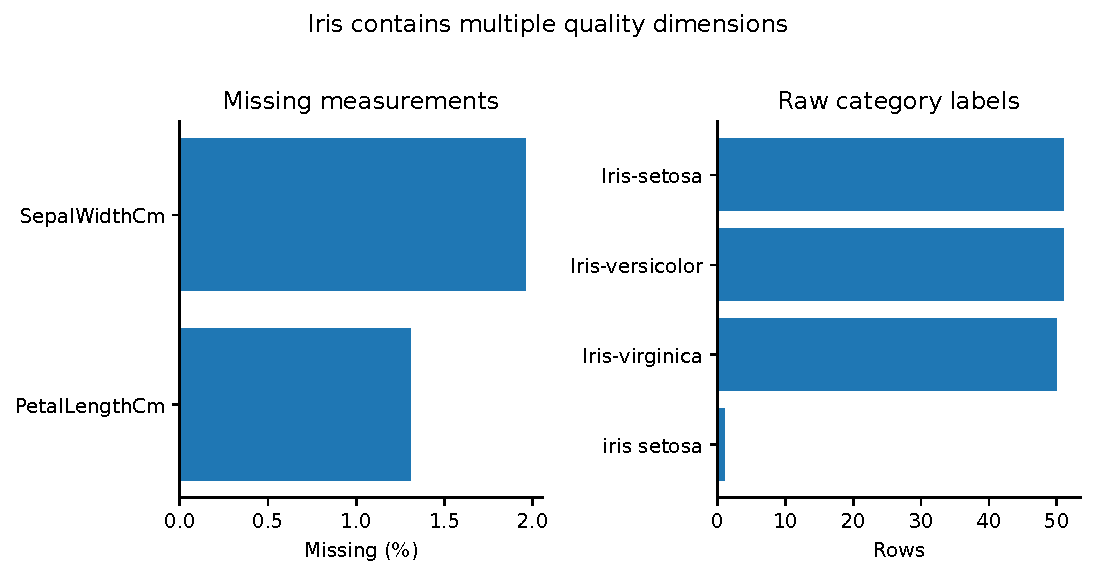
\includegraphics[width=0.88\linewidth]{figures_generated/quality_iris_audit.pdf}
\end{utpfig}

The 153-row Iris file contains three missing \texttt{SepalWidthCm} values, two missing \texttt{PetalLengthCm} values, and a lower-case/space variant of the setosa label. Converting labels to a canonical form is usually low-risk because the intended semantic equivalence is clear. Imputing a flower measurement is a stronger analytical decision because it invents a value and can change correlations, group means, or downstream classification.

\begin{utpfig}[Titanic missingness is concentrated, not uniform]{About 77\% of \texttt{Cabin} and 20\% of \texttt{Age} are missing, whereas most variables are complete. This pattern calls for variable-specific reasoning rather than a blanket ``drop missing rows'' rule.}{fig:quality-titanic-missing}
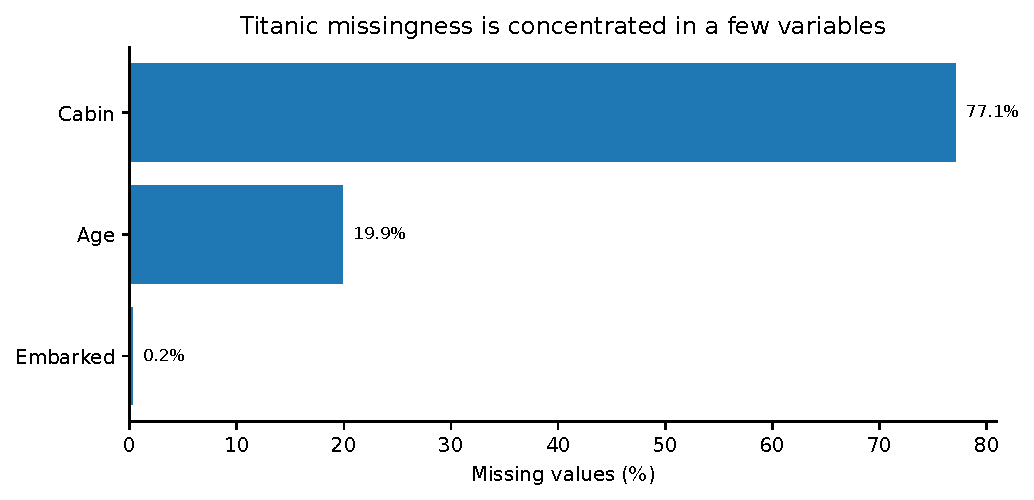
\includegraphics[width=0.82\linewidth]{figures_generated/quality_titanic_missingness.pdf}
\end{utpfig}

Deleting every row with any missing value would discard most passengers because \texttt{Cabin} is frequently absent. A professional audit asks what ``missing'' means: was a cabin never recorded, not applicable, unreadable in the source, or simply lost during data assembly? The answer determines whether missingness is nuisance, information, or both.

\begin{workedexample}
A sensible teaching strategy for \texttt{Age} is to preserve the original column and create \rcode{Age\_imputed}. Group-median imputation by passenger class and sex is transparent and reproducible, but it still shrinks within-group variation. The report should therefore state how many values were imputed and avoid presenting the derived ages as observed facts.
\end{workedexample}


\section{Extended audit: structural missingness and duplicate semantics}

The Ames Housing and Red Wine Quality datasets show why a professional data-quality review must go beyond a generic missing-value function. In Ames, some variables are almost entirely missing, but the reason is often structural: a property without a pool has no meaningful pool-quality rating, and a property without an alley cannot have an alley type. Encoding those cases as ordinary numeric or categorical missingness without understanding the data dictionary can erase information.

\begin{utpfig}[Ames missingness has semantic structure]{The most incomplete fields are largely optional property attributes. A high missing percentage is therefore a prompt to investigate meaning, not an automatic instruction to drop the column.}{fig:quality-ames-missing}
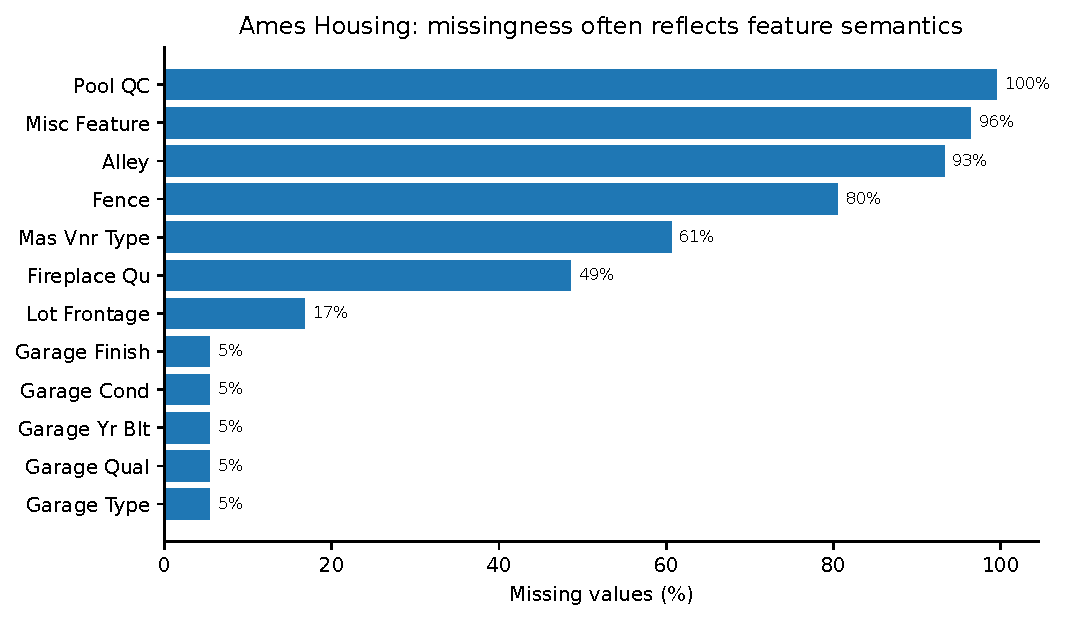
\includegraphics[width=0.86\linewidth]{figures_generated/quality_ames_missingness.pdf}
\end{utpfig}

This distinction is useful in modelling. For a feature such as \texttt{Pool QC}, an explicit category such as ``No pool'' can carry different information from ``pool quality was not recorded.'' The analyst should preserve that distinction whenever the source permits it.

The Red Wine Quality file illustrates a different issue. It contains exact duplicate rows even though no unique wine identifier is supplied.

\begin{utpfig}[Duplicate rows require a definition of the observational unit]{The file has fewer unique rows than supplied rows. That fact alone does not establish an error: two wines can share the same measured chemistry and quality score, or the same record may have been repeated.}{fig:quality-wine-duplicates}
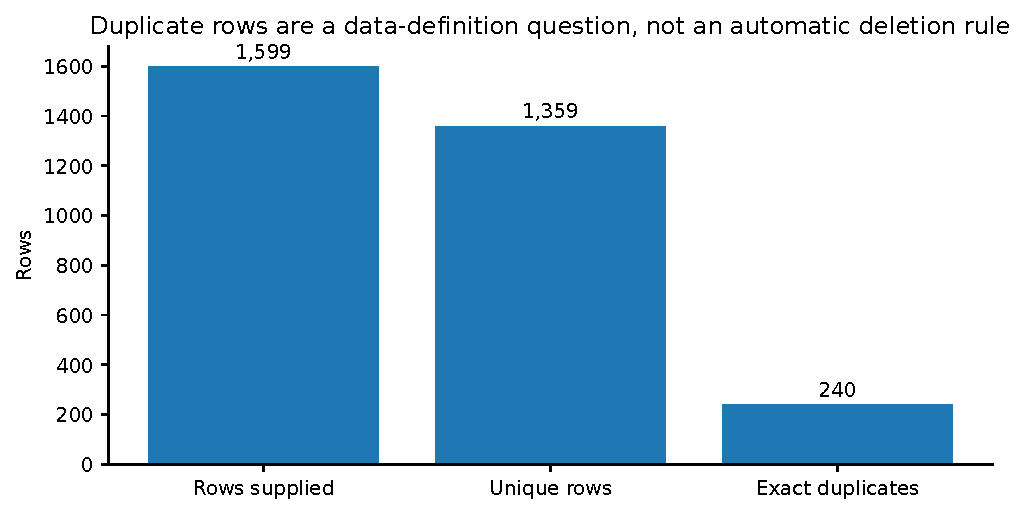
\includegraphics[width=0.72\linewidth]{figures_generated/quality_wine_duplicates.pdf}
\end{utpfig}

\begin{keyidea}
Never write \rcode{distinct()} or \rcode{duplicated()} as a cleaning ritual. First state the expected key and the intended unit of observation, then explain why repeated rows are impossible, possible, or informative under that definition.
\end{keyidea}

